\documentclass[11pt]{article}
\usepackage[utf8]{inputenc}	% Para caracteres en español
\usepackage{amsmath,amsthm,amsfonts,amssymb,amscd}
\usepackage{multirow,booktabs}
\usepackage[table]{xcolor}
\usepackage{fullpage}
\usepackage{lastpage}
\usepackage{enumitem}
\usepackage{fancyhdr}
\usepackage{mathrsfs}
\usepackage{wrapfig}
\usepackage{setspace}
\usepackage{hyperref}
\usepackage{calc}
\usepackage{multicol}
\usepackage{cancel}
\usepackage[retainorgcmds]{IEEEtrantools}
\usepackage[margin=3cm]{geometry}
\usepackage{amsmath}
\newlength{\tabcont}
\setlength{\parindent}{0.0in}
\setlength{\parskip}{0.05in}
\usepackage{empheq}
\usepackage{framed}
\usepackage[most]{tcolorbox}
\usepackage{xcolor}
\colorlet{shadecolor}{orange!15}
\parindent 0in
\parskip 12pt
\geometry{margin=1in, headsep=0.25in}
\theoremstyle{definition}
\usepackage{pdfpages}
\newtheorem{defn}{Definition}
\newtheorem{reg}{Rule}
\newtheorem{exer}{Exercise}
\newtheorem{note}{Note}
\usepackage{fancyhdr}\usepackage{xcolor}\usepackage{amsmath}\usepackage{amssymb}\pagestyle{fancy}\rhead{}
\newtheorem{theorem}{Theorem}[subsection]
\theoremstyle{definition}
\newtheorem{definition}[theorem]{Definiton}
\newtheorem{example}[theorem]{Example}
\newtheorem{corollary}[theorem]{Corollary}
\newtheorem{lemma}[theorem]{Lemma}
\title{Chapter 9 Review Notes}
\begin{document}
\thispagestyle{empty}
{\LARGE \bf MAT 292 Lecture Notes}\\
{\large Hei Shing Cheung}\\
Ordinary Differential Equations, Fall 2025 \hfill MAT292\\
\\
The up-to-date version of this document can be found at \url{https://github.com/HaysonC/skulenotes}\\

\begin{center}
    ``\textit{ODEs are the bread and butter of engineering. }''
\end{center}
\begin{shaded}
    \textbf{Key Concepts:}
    \begin{itemize}
        \item \textbf{Conflicting Definitions. } This course has multiple definitions for key terms, which may vary between different texts and contexts.
        \item \textbf{Practice Derivatives. } Regular practice with derivatives is essential for mastering ODEs.
        \begin{example}
            The following is a good example of good intuition:

            \textit{What is the antiderivative of $f(x) = \frac{\ln x}{x}$?}

            We know that this is of the form $g \cdot g'$where $g(x) = \ln x$ and $g'(x) = \frac{1}{x}$. Thus, by the rule that:

            \begin{equation}
            \frac{1}{2} \frac{d}{dx} [g(x)]^2 = g(x) g'(x)
            \end{equation}
            we can deduce that:
            $$
            \frac{1}{2} \frac{d}{dx} [(\ln x)^2] = \ln x \cdot \frac{1}{x}
            $$
        \end{example}
        \item \textbf{Practice Linear Algebra. } Familiarity with linear algebra concepts is crucial for understanding ODEs.
    \end{itemize}
\end{shaded}
\section{Examples and Review}
\subsection{What is a Differential Equation?}
\begin{definition}[Differential Equation]
     Any relationship between a variable and its derivatives is called a differential equation. 
\end{definition}

\begin{example}[Newton Second Law]
    Newton's second law states that the force acting on an object is equal to the mass of the object multiplied by its acceleration. Mathematically, this can be expressed as:
    $$
    F = m \frac{d^2x}{dt^2}
    $$
    where \( F \) is the force, \( m \) is the mass, and \( \frac{d^2x}{dt^2} \) is the acceleration (the second derivative of position with respect to time). This is a second-order ordinary differential equation.

    If force is constant, this is a simple form of a differential equation, which we simply rearrange and integrate it (twice), which gives, simply:
    $$
    x(t) = \frac{F}{2m} t^2 + C_1 t + C_0
    $$
    where \( C_1 \) and \( C_0 \) are constants determined by initial conditions.
\end{example}

\begin{example}
    Consider the following ODE:
    $$
    x' = f(t)
    $$
    So we have:
    $$
    \frac{dx}{dt} = f(t)
    $$
    Integrating both sides with respect to \( t \) gives:
    $$
    \int_0^t dx = \int_0^t f(t) \, dt
    $$
    So we have:
    $$
    x(t) = \int_0^t f(t) \, dt + C
    $$
    where \( C \) is a constant of integration. In which initial conditions can be used to determine the value of \( C \).  
\end{example}

\begin{example}[Standard Trick: Turning Higher Order into a System]
    Consider Hooke's Law:
    $$
    F = m\ddot{x} = -kx
    $$
    Then, we let:
    $$
    \begin{cases}
        x_1 = x \\
        x_2 = \dot{x} \\
        \dot{x}_1 = x_2 \\
        \dot{x}_2 = -\frac{k}{m} x_1
    \end{cases}
    $$
    This system can be solved using the techniques for first-order ODEs, as a system by its eigenvalues and eigenvectors:
    $$
    \begin{pmatrix}
        \dot{x}_1 \\
        \dot{x}_2
    \end{pmatrix}
    =
    \begin{pmatrix}
        0 & 1 \\
        -\frac{k}{m} & 0
    \end{pmatrix}
    \begin{pmatrix}
        x_1 \\
        x_2
    \end{pmatrix}
    $$
\end{example}

The above idea scales:

\begin{example}
    Take $F(t, x, \dot{x}, \ddot{x}, \ldots, x^{(n)}) = 0$. Then, we can let:
   \begin{equation}
    \begin{cases}
        x_1 = x \\
        x_2 = \dot{x} \\
        x_3 = \ddot{x} \\
        \vdots \\
        x_n = x^{(n)}
    \end{cases}
    $$
    This allows us to rewrite the original equation as a system of first-order equations:
    $$ 
    \begin{bmatrix}
        \dot{x}_1 \\
        \dot{x}_2 \\
        \vdots \\
        \dot{x}_n
    \end{bmatrix}
    =
    A
    \begin{bmatrix}
        x_1 \\
        x_2 \\
        \vdots \\
        x_n
    \end{bmatrix}
\end{equation}

Where we take $A$ to be the appropriate matrix.
\end{example}

\begin{example}[Exponential Growth]
    You should have already know, that:
    $$
    \frac{dx}{dt} = kx
    $$
    is a first-order linear ODE. The solution to this equation is given by:
    $$
    x(t) = Ce^{kt}
    $$
    where \( C \) is a constant determined by initial conditions.

We could understand the eigenproblems associated with systems of ODEs as an extension of the abovewhere we look for solutions of the form:
\begin{equation}
\begin{bmatrix}
x_1(t) \\
x_2(t) \\
\vdots \\
x_n(t)
\end{bmatrix}
=
e^{At}
\begin{bmatrix}
x_1(0) \\
x_2(0) \\
\vdots \\
x_n(0)
\end{bmatrix}
\end{equation}
where \( A \) is the matrix associated with the system of ODEs. $\exp(At)$ is the matrix exponential of \( At \), which can be computed using various methods, including power series or diagonalization.
\end{example}

\begin{example}[Superposition]
    You should also have already known that the solution to:
    $$ \ddot{x} = -x $$
    is given by:
    $$ x(t) = A \cos(t) + B \sin(t) $$
    where \( A \) and \( B \) are constants determined by initial conditions. The solutions $x_1 = A \cos(t)$ and $x_2 = B \sin(t)$ can be combined to form the general solution. Thus, additional conditions must be satisfied to determine the values of \( A \) and \( B \).
\end{example}
You might have observed that:
\begin{theorem}[Number of Initial Conditions]
    You need as many initial conditions as the order of the ODE to uniquely determine a solution.
\end{theorem}

\begin{example}[Newton's Law of Cooling]
    Let $u(t)$ be the temperature of the object at time $t$. Then, according to Newton's Law of Cooling, we have:
    $$
    \frac{du}{dt} = -k(u - T_a)
    $$
    where \( T_a \) is the ambient temperature, and \( k \) is a positive constant (the transmission coefficient). This is a first-order linear ODE that can be solved using the techniques discussed earlier.

    \textbf{Fixed-Point Solution} We denote the trivial case where \( u(0) = T_a \) as the fixed-point solutionwhere the temperature of the object is equal to the ambient temperature at time \( t = 0 \). It is easy to see that \( u' = 0 \) in this case so \( u(t) = T_a \) for all \( t \).

    One way of solving the general solution is:

    \begin{align*}
        \frac{du}{dt} &= -k(u - T_a) \\
        \int \frac{du}{u - T_a} &= -k \int dt \\
        \ln|u - T_a| &= -kt + C \\
        u - T_a &= e^C e^{-kt} \\
        u &= Be^{-kt} + T_a
    \end{align*}

\end{example}

\begin{definition}[Phase Portraits]
    A phase portrait is a graphical representation of the trajectories of a dynamical system in the phase plane. Each point in the phase plane corresponds to a unique state of the system, and the trajectories represent the evolution of the system over time. Phase portraits are useful for visualizing the behavior of systems of ODEs, particularly in understanding stability and equilibrium points.
\end{definition}

\subsection{Fixed Points}

We first consider the autonomous system:
\begin{equation}
    \frac{dx}{dt} = f(x)
\end{equation}

\begin{definition}[Autonomous System]
    An autonomous system is a system of ordinary differential equations (ODEs) in which the independent variable (usually time) does not explicitly appear in the equations. In other words, the rate of change of the dependent variable(s) depends only on the current state of the system and not on time itself. Autonomous systems can be expressed in the form:
    $$
    \frac{dx}{dt} = f(x)
    $$
    where \( x \) is the state vector and \( f(x) \) is a function that describes how the state changes over time.
\end{definition}

\begin{definition}[Fixed Point]
    A fixed point (or equilibrium point) of a dynamical system is a point in the phase space where the system remains unchanged over time. Mathematically, for a system described by the differential equation \( \frac{dx}{dt} = f(x) \), a fixed point \( x^* \) satisfies:
    $$
    f(x^*) = 0
    $$
    This means that if the system starts at \( x^* \), it will stay at \( x^* \) for all future times.
\end{definition}

\begin{example}
    Consider $x' = \sin(x)$. The fixed points are given by:
    $$
    \sin(x) = 0 \implies x = n\pi, \quad n \in \mathbb{Z}
    $$
    Thus, the fixed points are \( x = 0, \pm \pi, \pm 2\pi, \ldots \)
\end{example}

\subsubsection{Stability of Fixed Points}
\paragraph{Intuition} Consider a simple pendulum parametized by the angle \( \theta \) from the vertical. The fixed points of this system occur when the pendulum is at rest, which happens at \( \theta = 0 \) (hanging straight down) and \( \theta = \pi \) (inverted position). The case where \textbf{\( \theta = 0 \) is stable}, as small perturbations will cause the pendulum to oscillate around this point. In contrast, \textbf{\( \theta = \pi \) is unstable,} as any small perturbation will cause the pendulum to fall away from this position.

\paragraph{What determines stability?} A fixed point \( x^* \) of a dynamical system \( \frac{dx}{dt} = f(x) \) is classified as:

\begin{subequations}
    stable if:
    \begin{equation}
        \frac{df}{dx} \bigg|_{x=x^*} < 0
    \end{equation}
    unstable if:
    \begin{equation}
        \frac{df}{dx} \bigg|_{x=x^*} > 0
    \end{equation}
    semi-stable if:
    \begin{equation}
        \frac{df}{dx} \bigg|_{x=x^*} = 0
    \end{equation}
\end{subequations}

\begin{proof}
    A demonstration of this will be given in the next section on Linear Stability Analysis \ref{def:linear-stability-analysis}.
\end{proof}

\begin{example}
    Consider the system $x' = \sin(x)$. The fixed points are at \( x = n\pi \)where \( n \in \mathbb{Z} \). To determine the stability of these fixed points, we compute the derivative of \( f(x) = \sin(x) \):
    $$
    \frac{df}{dx} = \cos(x)
    $$
    Evaluating this derivative at the fixed points $x = n\pi$ gives:
    $$
    \cos(n\pi) =\begin{cases}
        1 & \text{if } n \text{ is even (unstable)} \\
        -1 & \text{if } n \text{ is odd (stable)}
    \end{cases}
    $$
    Thus, the fixed points at \( x = 0, \pm 2\pi, \pm 4\pi, \ldots \) are unstable, while the fixed points at \( x = \pm \pi, \pm 3\pi, \pm 5\pi, \ldots \) are stable. 
\end{example}

\paragraph{Drawing Fixed Point Diagrams and Phase Portraits} By visualizing the direction of $x$ due to $x' = f(x)$ on a $x$, $f(x)$ plane (fixed points diagram), we can draw a phase portrait. For the phase portrait, we can demonstrate the fixed points as horizontal lines, and draw points of $x$ that converge to or diverge from these fixed points according to the direction of $x'$.

We draw the fixed point diagram with filled circles for stable fixed points and open circles for unstable fixed points. Arrows indicate the direction of flow towards or away from the fixed points.

\begin{figure}[h!]
    \centering
    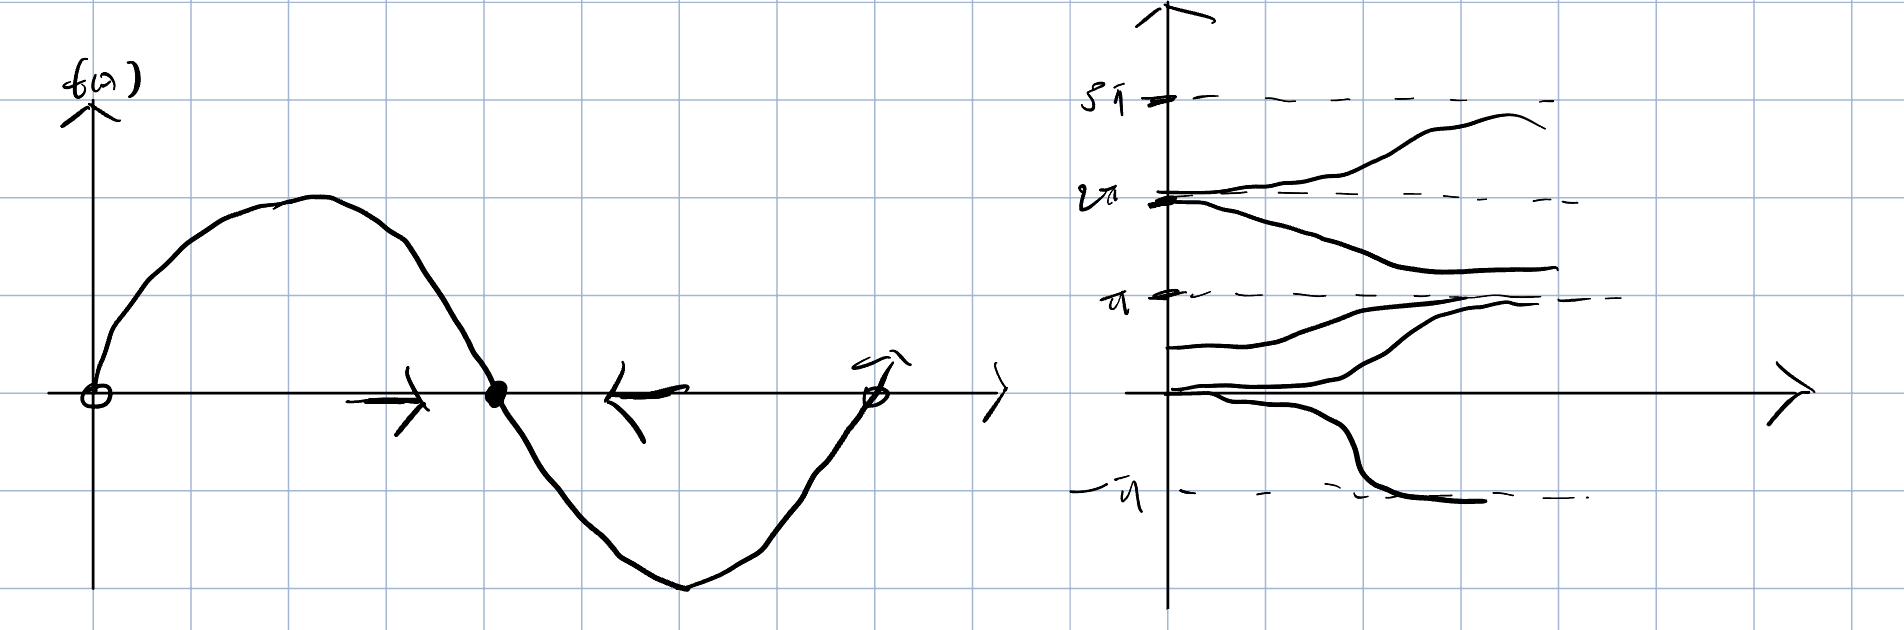
\includegraphics[width=0.6\textwidth]{fixpointdiagram.jpeg}
    \caption{Fixed Point Diagram and Phase Portrait for \( x' = \sin(x) \)}
    \label{fig:fixpointdiagram}
\end{figure}

\begin{theorem}[Non-Intersection of Solutions]
    In a dynamical system described by an ordinary differential equation (ODE) with a unique solution for given initial conditions, the trajectories of different solutions cannot intersect in the phase space. This means that if two solutions start from different initial conditions, they will never cross each other at any point in time.
\end{theorem}
\begin{proof}
    \textbf{Sketch:} If the solutions intersect, then at the point of intersection, the solution is not unique, which contradicts the assumption of uniqueness.
\end{proof}


\paragraph{What Happens When We Consider $t \to -\infty$?} 
\begin{theorem}[Stability Reversal]
    A fixed point that is stable as \( t \to \infty \) becomes unstable as \( t \to -\infty \), and vice versa.
\end{theorem}

\begin{proof}
    This can be understood by considering the time-reversed system. If we denote the time-reversed variable as \( t' = -t \), then the original system \( \frac{dx}{dt} = f(x) \) transforms, by the chain rule, into:
    $$
    \frac{dx}{dt'} = -f(x) 
    $$
    In this new system, the direction of flow is reversed. Therefore, if a fixed point \( x^* \) is stable in the original system (i.e., trajectories approach \( x^* \) as \( t \to \infty \)), it will be unstable in the time-reversed system (i.e., trajectories move away from \( x^* \) as \( t' \to \infty \)). Conversely, an unstable fixed point in the original system becomes stable in the time-reversed system. This demonstrates the reversal of stability when considering \( t \to -\infty \).
\end{proof}
    

\subsubsection{Linear Stability Analysis}

\begin{definition}[Linear Stability Analysis] \label{def:linear-stability-analysis}
    Consider the system $x' = f(x)$. Let $\epsilon$ be any perturbation around a fixed point $x^*$, such that:
    $$x = x^* + \epsilon
    $$
    To analyze the stability of the fixed point, we analyze the behavior of the perturbation $\epsilon(t)$ over time, since $x^*$ is fixed, we have:
    \begin{align*}
        \epsilon' = x' = f(x) &= f(x^* + \epsilon) \\
        \intertext{Ignoring higher order terms in Taylor expansion, we have:}
        &\approx f(x^*) + \epsilon f'(x^*) + \cancel{\frac{1}{2} \epsilon^2 f''(x^*) + \ldots} \\
        &= \epsilon f'(x^*) \quad \text{(since } f(x^*) = 0 \text{)} \\
        \Rightarrow \epsilon' &= f'(x^*) \epsilon
    \end{align*}

    This is a linear ODE in $\epsilon$, which can be solved as:
    $$\epsilon(t) = \epsilon e^{f'(x^*) t}
    $$
    The behavior of $\epsilon(t)z$ depends on the sign of $f'(x^*)$:
    \begin{itemize}
        \item If $f'(x^*) < 0$, then $\epsilon(t) \to 0$ as $t \to \infty$, indicating that the fixed point is stable.
        \item If $f'(x^*) > 0$, then $\epsilon(t) \to \infty$ as $t \to \infty$, indicating that the fixed point is unstable.
        \item If $f'(x^*) = 0$, the linear analysis is inconclusive, and higher-order terms must be considered.
    \end{itemize}
    Thus, the stability of the fixed point can be determined by the sign of $f'(x^*)$.
\end{definition}

\begin{example}
    Consider the system $x' =x^2$. The only fix point is at \( x = 0 \). We have $f'(x) = 2x$, and at the fixed point:
    $$
    f'(0) = 0
    $$
    Thus, the linear stability analysis is inconclusive. We draw the fixed point half filled on the left, and half empty on the right. This is becuase for \( x < 0 \), \( f(x) = x^2 > 0 \), so points to the left of the fixed point move away from it (unstable). For \( x > 0 \), \( f(x) = x^2 > 0 \), so points to the right of the fixed point also move away from it (unstable). Therefore, the fixed point at \( x = 0 \) is unstable.
\end{example}

\subsection{Classification of ODEs}

\begin{shaded}
\paragraph{ODE vs PDE} An ordinary differential equation (ODE) contains functions of a single variable and their derivatives. A partial differential equation (PDE) contains functions of multiple variables and their partial derivatives.
\begin{example}[Heat Equation]
    The heat equation is a PDE that describes how heat diffuses through a given region over time. It is given by:
    $$
    \frac{\partial u}{\partial t} = \alpha \nabla^2 u 
    $$
    where \( u(x, t) \) is the temperature distribution function, \( \alpha \) is the thermal diffusivity constant, and \( \nabla^2 \) is the Laplacian operator.
\end{example}
\begin{example}[Laplace's Equation]
    Laplace's equation is a PDE that describes the behavior of scalar fields such as electric potential and fluid flow. It is given by:
    $$
    \nabla^2 \phi = 0
    $$
    where \( \phi(x, y, z) \) is the scalar potential function, and \( \nabla^2 \) is the Laplacian operator.
    
\end{example}
\end{shaded}
\begin{definition}[Order of an ODE]
    The order of an ordinary differential equation (ODE) is determined by the highest derivative present in the equation.
\end{definition}
\subsubsection{Linearity and Homogeneity of ODEs}
\begin{definition}[Linearity of an ODE]
    An ordinary differential equation (ODE) is considered linear if it can be expressed in the form:
    $$
    a_n(x) \frac{d^n y}{dx^n} + a_{n-1}(x) \frac{d^{n-1} y}{dx^{n-1}} + \ldots + a_1(x) \frac{dy}{dx} + a_0(x) y = g(x)
    $$
    where \( y \) is the dependent variable, \( x \) is the independent variable, \( a_i(x) \) are functions of \( x \), and \( g(x) \) is a known function. In a linear ODE, the dependent variable \( y \) and its derivatives appear to the first power and are not multiplied together. Otherwise, the ODE is considered nonlinear.    
\end{definition}

\begin{definition}[Homogenity of Linear ODEs]
    A linear ordinary differential equation (ODE) is said to be homogeneous if the function \( g(x) \) on the right-hand side of the equation is equal to zero for all values of \( x \). In other words, a homogeneous linear ODE has the form:
    $$
    a_n(x) \frac{d^n y}{dx^n} + a_{n-1}(x) \frac{d^{n-1} y}{dx^{n-1}} + \ldots + a_1(x) \frac{dy}{dx} + a_0(x) y = 0
    $$
    If \( g(x) \) is not identically zero, then the ODE is considered non-homogeneous. Homogeneous linear ODEs have special properties and solution methods that differ from those of non-homogeneous linear ODEs.
\end{definition}

\begin{theorem}[Principle of Superposition]
    Let:
    $$
    a_0(t)y + \dots + a_n(t) \frac{d^n y}{dt^n} =0
    $$
    Assuming that $y_1(t)$ and $y_2(t)$ are two solutions to the above equation, then any linear combination of these solutions $A y_1(t) + B y_2(t)$, where \( A \) and \( B \) are constants, is also a solution.
\end{theorem}
\begin{proof}
    This could be demonstrated by the following derivation:
    \begin{align*}
        & a_0(t)(A y_1 + B y_2) + \dots + a_n(t) \frac{d^n}{dt^n}(A y_1 + B y_2) \\ 
        &= A \left( a_0(t)y_1 + \dots + a_n(t) \frac{d^n y_1}{dt^n} \right) + B \left( a_0(t)y_2 + \dots + a_n(t) \frac{d^n y_2}{dt^n} \right) \\
        &= A \cdot 0 + B \cdot 0 \\
        &= 0
    \end{align*}
    Thus, \( A y_1(t) + B y_2(t) \) is also a solution to the original equation. WLOG, this can be extended to any finite number of solutions.
\end{proof}

Conisder the non-homogeneous case:
\begin{theorem}[General Solution of Non-Homogeneous Linear ODEs]
    Let:
    $$
    a_0(t)y + \dots + a_n(t) \frac{d^n y}{dt^n} =g(t)
    $$
    If \( y_p(t) \) is a particular solution to the non-homogeneous equation, and \( y_h(t) \) is any solution to the corresponding homogeneous equation, then:
    $$
    y(t) = A y_h(t) + y_p(t)
    $$
    is the general solution to the non-homogeneous equation, where \( A \) is an arbitrary constant.
\end{theorem}
\begin{proof}
    \textbf{Sketch:} The solution for the homogeneous part would simply be 0, so the particular solution would be the only solution to the non-homogeneous equation. The general solution is then the sum of the homogeneous and particular solutions.
\end{proof}

\subsubsection{Separable ODEs}
\begin{definition}[Separable ODE]
    An ordinary differential equation (ODE) is said to be separable if it can be expressed in the form:
    $$
    \frac{dy}{dx} = g(x) h(y) = f(x, y)
    $$
    where \( g(x) \) is a function of the independent variable \( x \) only, and \( h(y) \) is a function of the dependent variable \( y \) only. This allows the variables to be separated on opposite sides of the equation, enabling integration with respect to each variable independently:

    \begin{align*}
        \frac{dy}{dx} &= g(x) h(y) \\
        \int \frac{1}{h(y)} dy &= \int g(x) dx \\
        \intertext{Let \( H(y) \) be the antiderivative of \( \frac{1}{h(y)} \) and \( G(x) \) be the antiderivative of \( g(x) \), we have:}
        H(y) &= G(x) + C \\
        \Rightarrow y &= H^{-1}(G(x) + C)
    \end{align*}
    where \( C \) is the constant of integration.
\end{definition}

\paragraph{Remarks} If $g$ and $h$ are continuous, then there need not exist solution in a neighbourhood (open $\epsilon$-ball) of any point $(x_0, y_0)$ so long as $h(y_0) \neq 0$.

\begin{example}
    Consider the IVP:
    $$
    \begin{cases}
        \frac{dx}{dt} = ax \\
        x(0) = x_0
    \end{cases}
    $$
    then the solution is given by:
    $$
    x(t) = x_0e^{at}
    $$
    Is the solution unique? Suppose $x$ is any solution, then we check if $y = e^{-at}x$ is constant:
    \begin{align*}
        \frac{dy}{dt} &= \frac{d}{dt}(e^{-at}x) \\
        &= -ae^{-at}x + e^{-at}\frac{dx}{dt} \\
        &= -ae^{-at}x + e^{-at}(ax) \\
        &= 0
    \end{align*}
    Thus, $y$ is constant, and since $y(0) = x_0$, we have $y(t) = x_0$ for all $t$. Thus,
    $$x(t) = x_0 e^{at}
    $$
    which is the unique solution.
\end{example}

\begin{example}[Logistic Equation]
    The logistic equation is a first-order nonlinear separable autonomous ODE that models population growth with a carrying capacity. It is given by:
    $$
    \frac{dx}{dt} = \alpha x \left(1 - x \right)
    $$
    where \( \alpha \) is the growth rate.

    To solve this equation, we can separate the variables:
    \begin{align*}
        \frac{dx}{\alpha x(1 - x)} &= 1 dt \\
        \int \frac{1}{\alpha x(1 - x)} dx &= \int 1 dt \\
        \intertext{Using partial fraction decomposition, we have:}
        \frac{1}{\alpha x(1 - x)} &= \frac{A}{x} + \frac{B}{1 - x} \\
        1 &= A(1 - x) + Bx \\
        1 &= A + (B - A)x \\
        \Rightarrow A &= 1, \quad B - A = 0 \\
        \Rightarrow B &= 1
        \intertext{Thus, we have:}
        \int \left( \frac{1}{\alpha x} + \frac{1}{\alpha (1 - x)} \right) dx &= \int 1 dt \\
        \frac{1}{\alpha} \left( \ln|x| - \ln|1 - x| \right) &= t + C \\
        \ln \left| \frac{x}{1 - x} \right| &= \alpha t + C' \\
        \frac{x}{1 - x} &= e^{\alpha t + C'} = Ce^{\alpha t} \\
        \Rightarrow x(t) &= \frac{Ce^{\alpha t}}{1 + Ce^{\alpha t}}
    \end{align*}

    To analyze the stability of the fixed points, we first find the fixed points by setting \( \frac{dx}{dt} = 0 \):
    $$\alpha x(1 - x) = 0 \implies x = 0 \text{ or } x = 1
    $$
    Next, we compute the derivative of \( f(x) = \alpha x(1 - x) \):
    $$\frac{df}{dx} = \alpha (1 - 2x)
    $$
    Evaluating this derivative at the fixed points, assumeing \( \alpha > 0 \):
    \begin{itemize}
        \item At \( x = 0 \):
        $$\frac{df}{dx} \bigg|_{x=0} = \alpha > 0 \quad \text{(unstable)}
        $$
        \item At \( x = 1 \):
        $$\frac{df}{dx} \bigg|_{x=1} = -\alpha < 0 \quad \text{(stable)}
        $$
    \end{itemize}
    Thus, the fixed point at \( x = 0 \) is unstable, while the fixed point at \( x = 1 \) is stable.
\end{example}
\end{document}